\documentclass[a4paper]{article}
\usepackage{graphicx}
\usepackage{fancyhdr}
\usepackage{geometry}
\geometry{
	a4paper,
	total={170mm,257mm},
	left=20mm,
	top=20mm,
	bottom=39mm,
}

\setlength{\headheight}{82.70538pt}

\fancypagestyle{oida}{
	\fancyhf{}
	\fancyhead[L]{\fontsize{7.5}{7.5}htl donaustadt\\ Donaustadtstraße 45\\
		1220 Wien\\~\\ Abteilung: Informationstechnologie\\ 
	Schwerpunkt: Netzwerktechnik}
	\fancyhead[R]{
\includegraphics[scale=0.45]{logo.png}}

	\fancyfoot[L]{\today}
	\fancyfoot[C]{\jobname}
	\fancyfoot[R]{Seite: \thepage}
}

\begin{document}
\pagestyle{oida}
\section*{Thema}
\par\noindent\rule{\textwidth}{0.4pt}

Laborprotokoll
TCP-UPD Header Verleich

\begin{figure}[h]
	
\includegraphics[scale=0.6]{meme.jpeg}
	\caption{memes klauen ist nicht ethisch}
\end{figure}

\vspace*{\fill}
Unterrichtsgegenstand:	NWT1|ZIVK

Jahrgang:	2BHIT

Name:	Stefan Fürst

Betreuer: 	ZIVK

Übungsdaten:	24.5.2024

Abgabedatum:	Datum


\newpage
\tableofcontents

\newpage

\section{Aufgabenstellung}
TCP-UDP Header vergleich.
\section{Zusammenfassung}
Netcad um einen TCP/UPD Server starten, mit Netcad verbinden und mit Wireshark die Verbindungen analysieren.

\newpage

\section{Vollständige Netzwerktopologie der gesamten Übung}

\newpage

\section{Übungsdurchführung}

\subsection{Aufsetzen der Server}
%command für das ding mit code block schön machen
\paragraph{TCP}
nc -l -p 5000
\paragraph{UDP}
nc -l -u -p 5000

\subsubsection{Verbinden mit dem Sever (TCP)}
nc 10.23.38.117 4201
\subsubsection{TCP-Verbindungsaufbau}
\begin{figure}[h]
	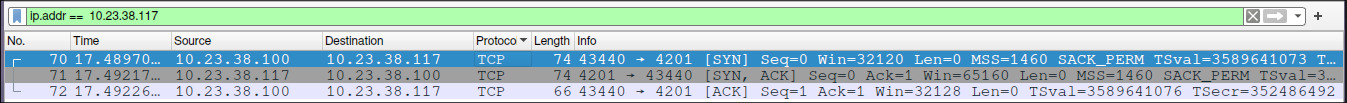
\includegraphics[scale=0.6]{images\handshake.jpeg}
	\caption{TCP 3 Way Handshake}
\end{figure}
\subsubsection{Nachrichten verschicken und empfangen}
\begin{figure}[h]
	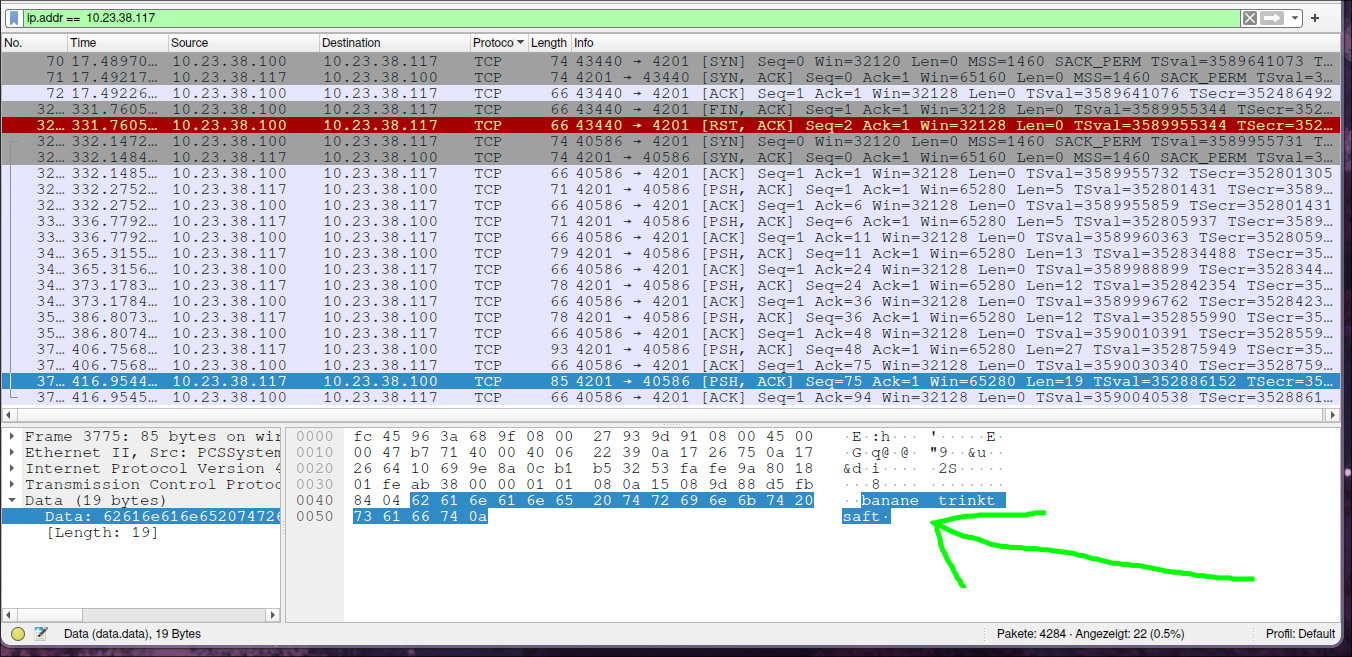
\includegraphics[scale=0.6]{images\nachricht.jpeg}
	\caption{Nachricht}
\end{figure}
\subsubsection{TCP-Flags}
% https://www.geeksforgeeks.org/tcp-flags/
% den schaß citen
TCP-Flags dienen dazu um den Zustand, oder andere zusätzliche Informationen der Verbindung anzuzeigen.\\
Diese diesen zum Troubleshooten.
\begin{figure}[h]
	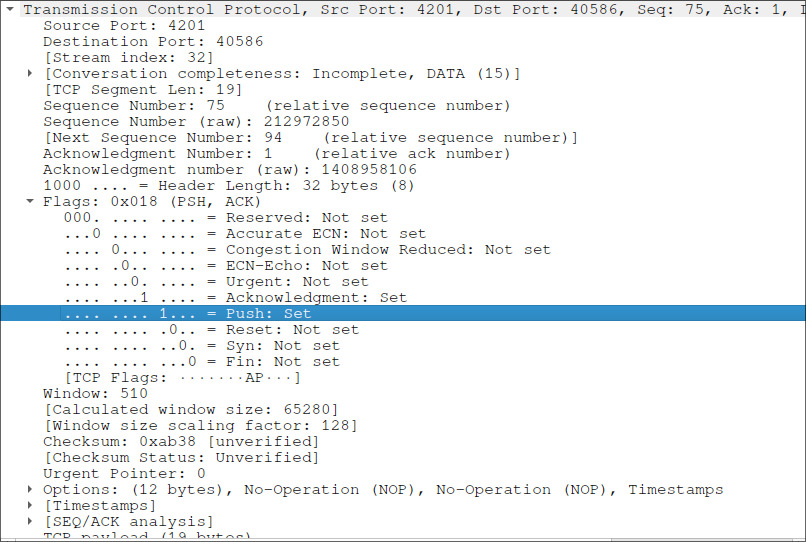
\includegraphics[scale=0.6]{images\tcp-flags.jpeg}
	\caption{TCP-Flags}
\end{figure}
In der Übung ist die Push flag gesetzt, was bedeuted, dass die Nachricht sofort übertragen wird, ohne darauf zu warten, dass zusätliche Informationen auf der Senderseite gebuffert werden.
\\ Wird oft in Echtzeitapplikation benutzt.
\subsubsection{TCP-Header}
\begin{figure}[h]
	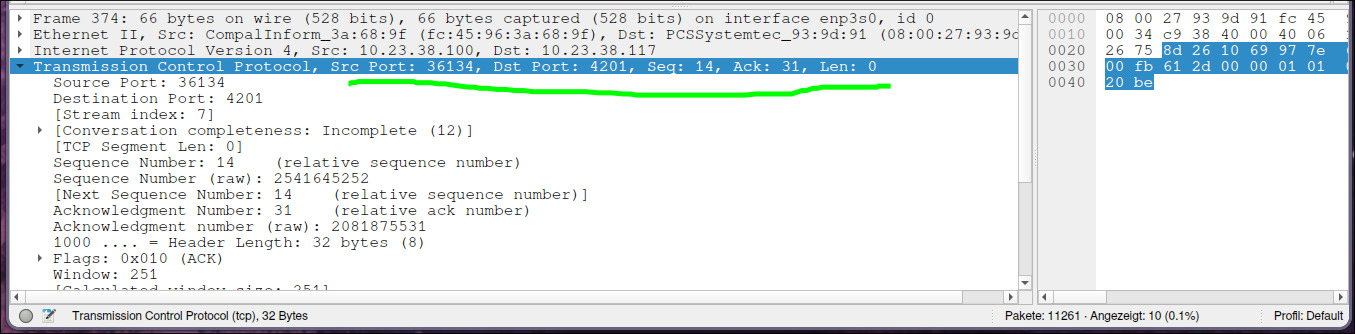
\includegraphics[scale=0.6]{images\tcp-header.jpeg}
	\caption{TCP-Header}
\end{figure}
\subsubsection{Verbinden mit dem Sever (UDP)}
nc -u 10.23.38.117 4201
\subsubsection{UDP-Verbindungsaufbau}
\begin{figure}[h]
	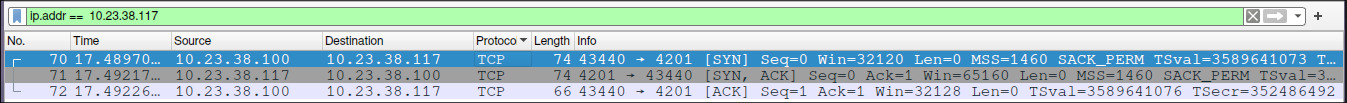
\includegraphics[scale=0.6]{images\handshake.jpeg}
	\caption{TCP 3 Way Handshake}
\end{figure}
\subsubsection{Nachrichten verschicken und empfangen}
\begin{figure}[h]
	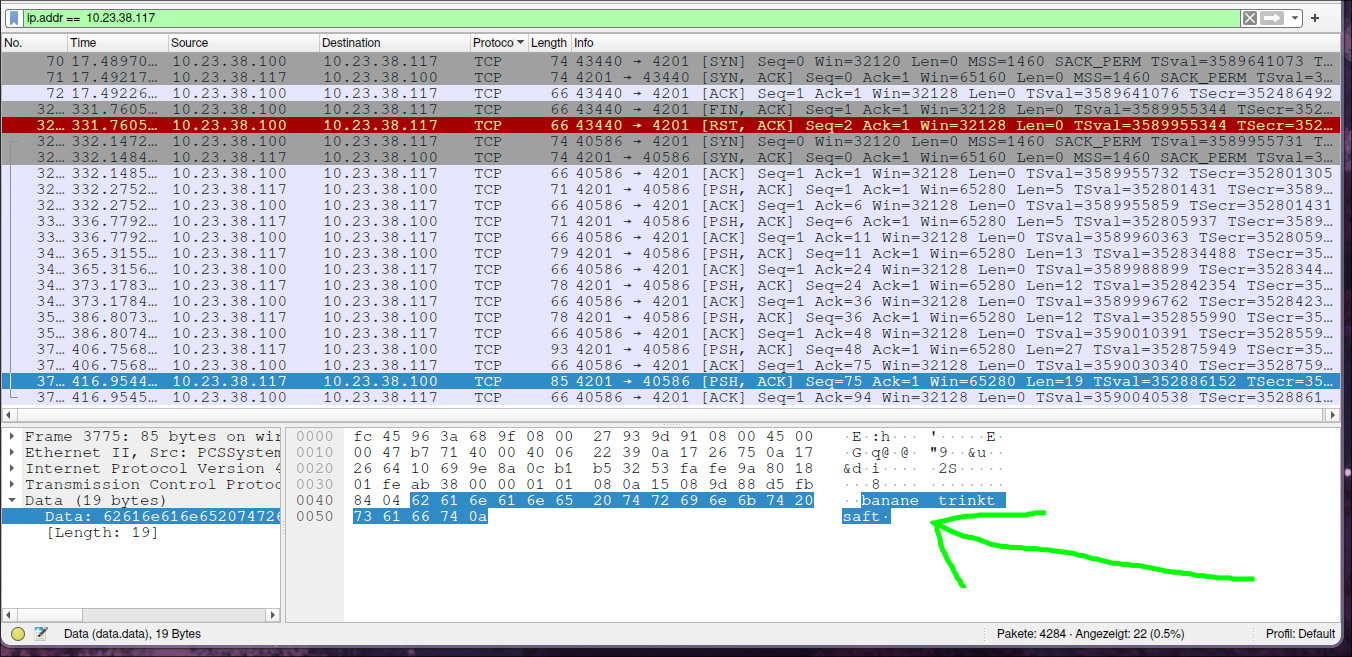
\includegraphics[scale=0.6]{images\nachricht.jpeg}
	\caption{Nachrichten}
\end{figure}
\newpage

\section{Vollständige Konfigurationsdatein}

\newpage

\section{Abbildungsverzeichnis}

\listoffigures

\end{document}
